% \chapter{The first appendix}

% Text for the first appendix goes here.

% \section{Appendix section}

% Text for a section in the first appendix goes here.

% test ทดสอบฟอนต์ serif ภาษาไทย

% \textsf{test ทดสอบฟอนต์ sans serif ภาษาไทย}

% \verb+test ทดสอบฟอนต์ teletype ภาษาไทย+

% \texttt{test ทดสอบฟอนต์ teletype ภาษาไทย}

% \textbf{ตัวหนา serif ภาษาไทย \textsf{sans serif ภาษาไทย} \texttt{teletype ภาษาไทย}}

% \textit{ตัวเอียง serif ภาษาไทย \textsf{sans serif ภาษาไทย} \texttt{teletype ภาษาไทย}}

% \textbf{\textit{ตัวหนาเอียง serif ภาษาไทย \textsf{sans serif ภาษาไทย} \texttt{teletype ภาษาไทย}}}

% \url{https://www.example.com/test_ทดสอบ_url}

\chapter{\ifenglish Manual\else คู่มือการใช้งานระบบ\fi}
% begin itemize with number
\begin{itemize}
    \item \textbf{การใช้งานในส่วนของ User ทั่วไป}
\begin{enumerate}
    \item ทำการ Login เข้าสู่ระบบผ่าน CMU Account หรือ สามารถค้นหาโปรเจ็คได้โดยไม่ต้อง Login 
    % make it to call image
    \begin{figure}[H]
    \centering
    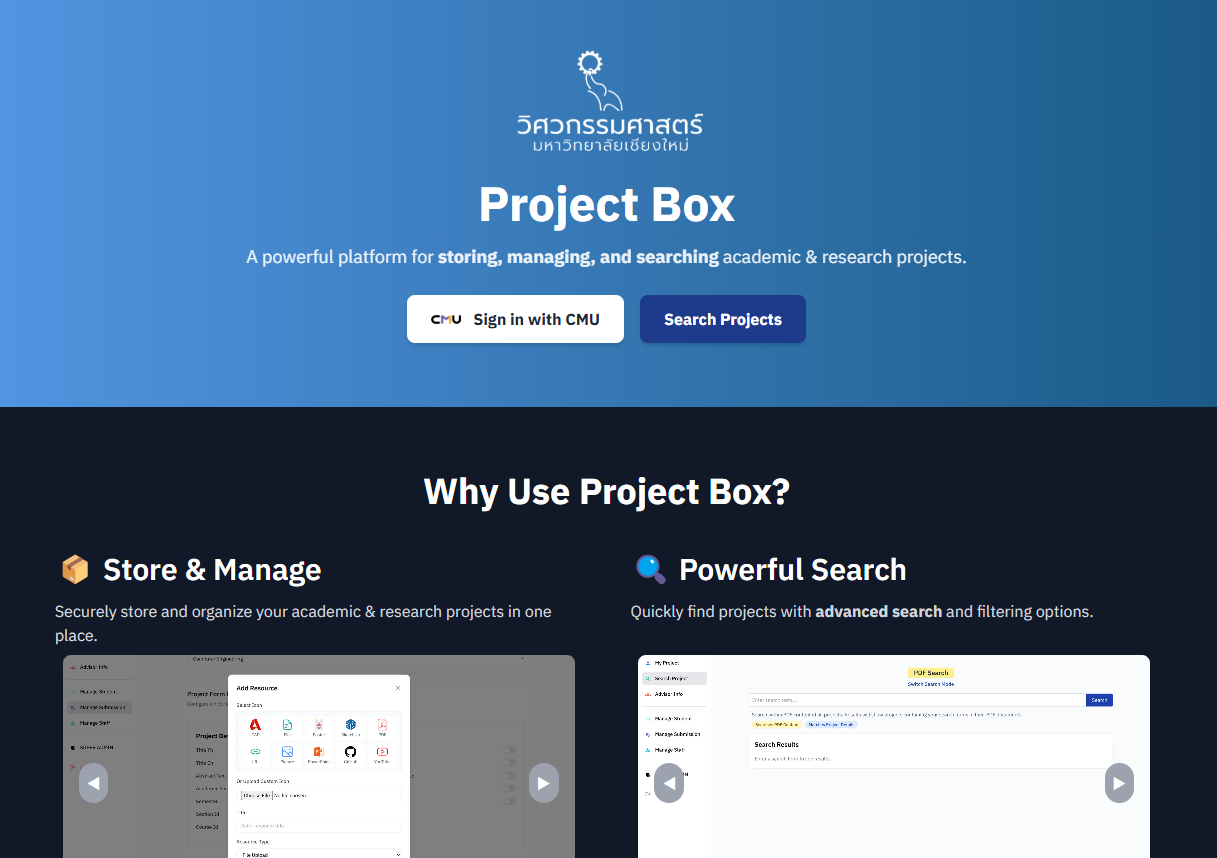
\includegraphics[width=130mm, keepaspectratio ]{pictures/project_box/loginpage.png}
    \end{figure}
    % space between image and text
    \vspace{1cm}
    \item เมื่อทำการ Login สำเร็จ จะเข้าสู่หน้า Dashboard ที่แสดงโปรเจ็คที่เคยสร้างไว้แล้ว หรือสามารถสร้างโปรเจ็คใหม่ได้เมื่อมีการลงทะเบียนเข้าใช้งาน
    \begin{figure}[H]
        \centering
        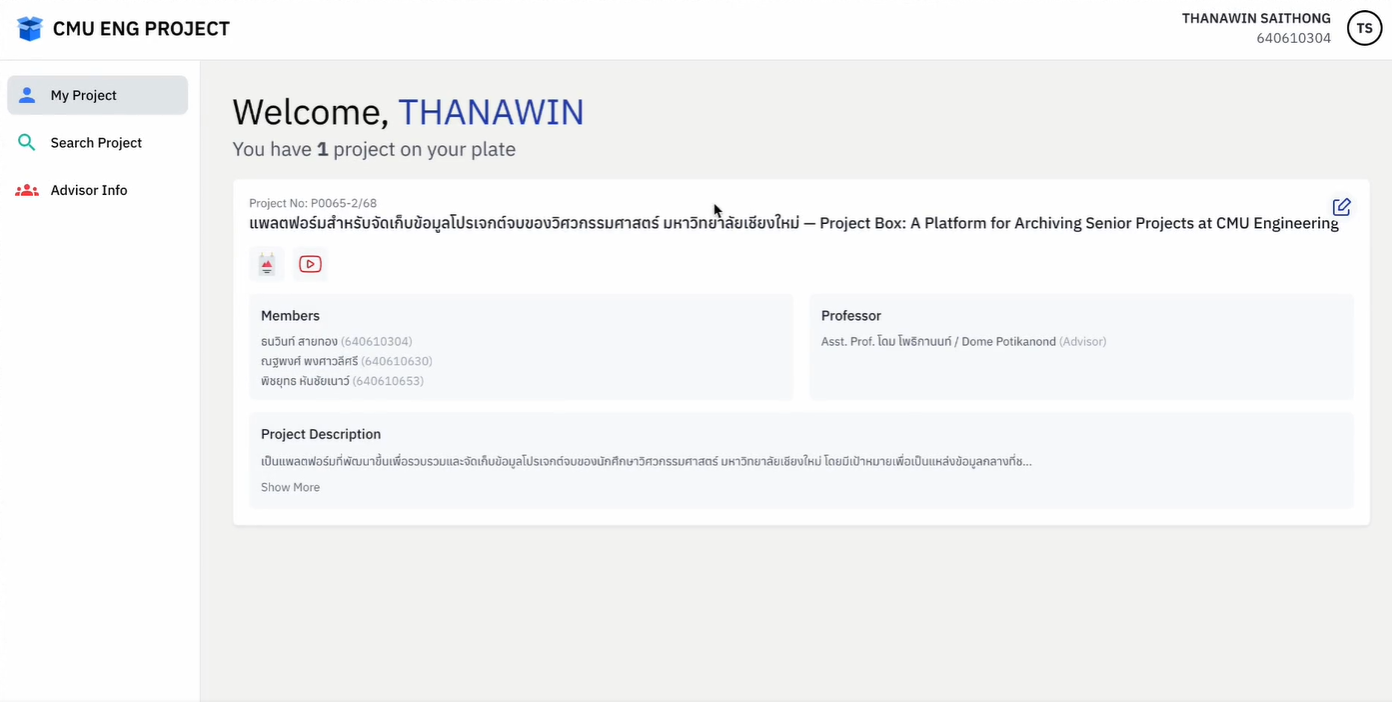
\includegraphics[width=130mm, keepaspectratio ]{pictures/project_box/dashboard.png
        }
    \end{figure}
    % new page after this 
    \newpage
    \item การค้นหาโปรเจ็ค สามารถค้นหาโปรเจ็คที่ต้องการได้จากช่องค้นหาโครงงาน 
    \begin{enumerate}
        \item Qucik Search ใช้การค้นหาโครงงานแบบง่าย
        \begin{figure}[H]
            \centering
            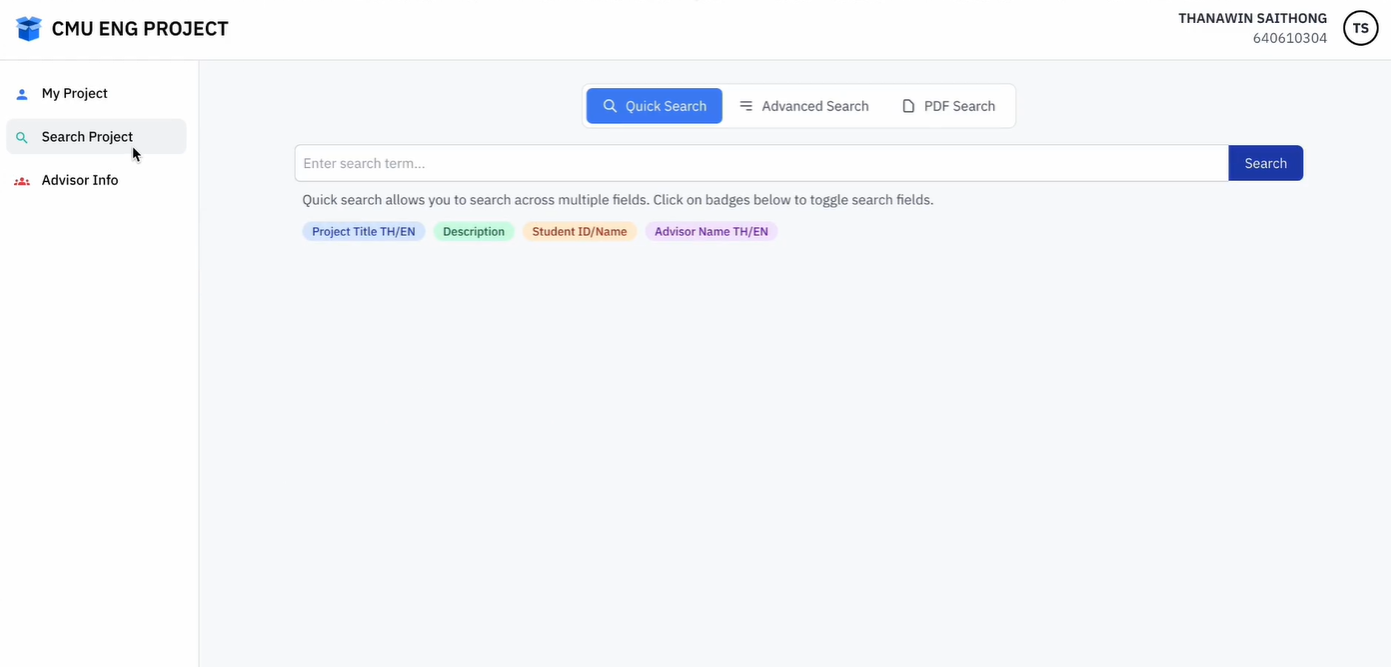
\includegraphics[width=130mm, keepaspectratio ]{pictures/project_box/quick_search.png}
        \end{figure}
        \item Advanced Search ใช้การค้นหาโครงงานแบบละเอียด
        \begin{figure}[H]
            \centering
            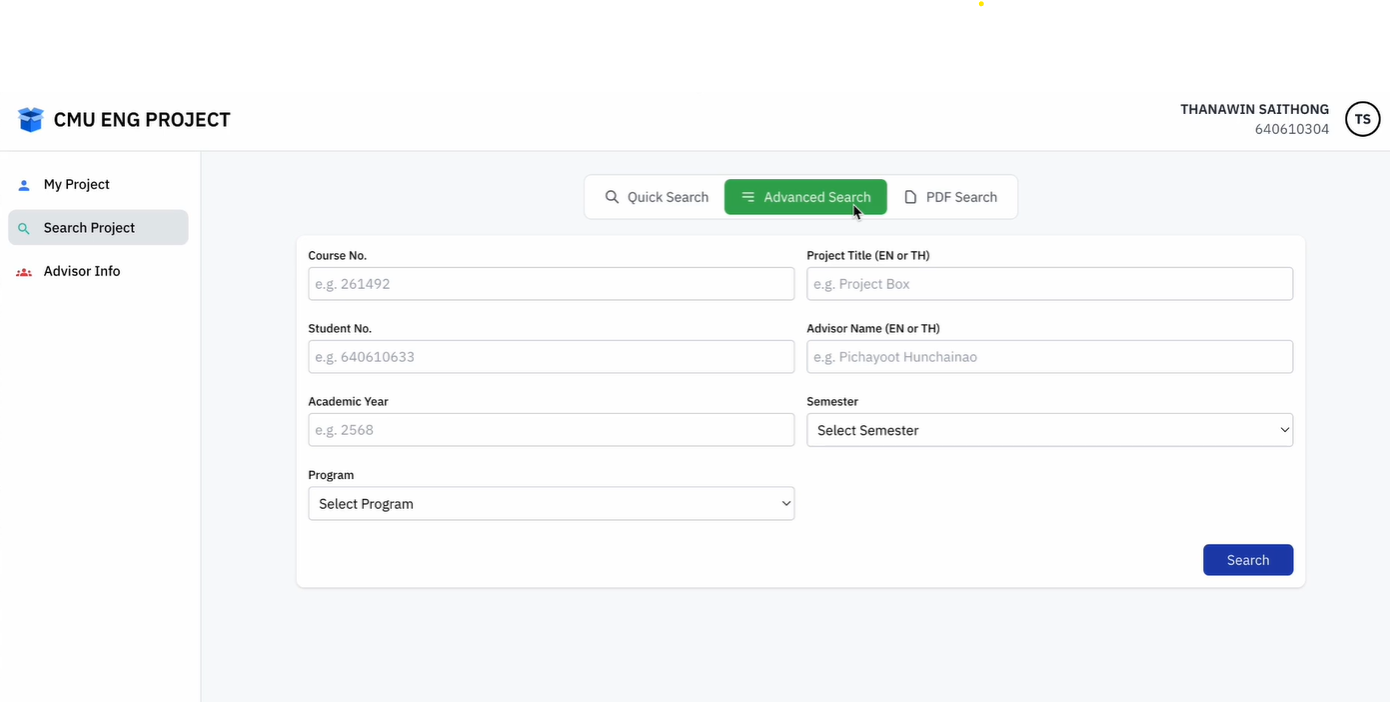
\includegraphics[width=130mm, keepaspectratio ]{pictures/project_box/advance_search.png}
        \end{figure} 
        \item PDF Search ใช้การค้นหาโครงงานจากไฟล์ PDF
        \begin{figure}[H]
            \centering
            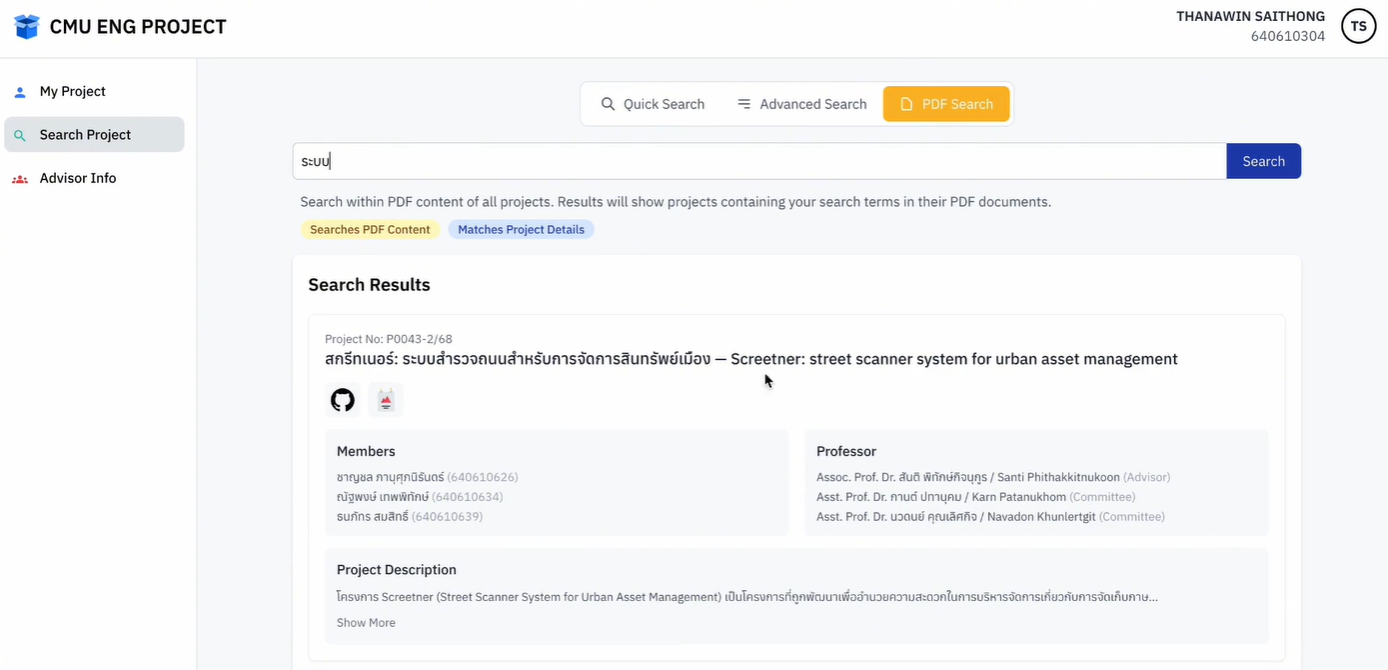
\includegraphics[width=130mm, keepaspectratio ]{pictures/project_box/pdf_search.png}
        \end{figure} 
    \end{enumerate}
    \item ค้นหา Advisor Information สามารถค้นหาข้อมูลของอาจารย์ที่เกี่ยวข้องกับโครงงานได้
    \begin{enumerate}
        \item เลือกสาจารย์ที่ต้องการค้นหา
        \begin{figure}[H]
            \centering
            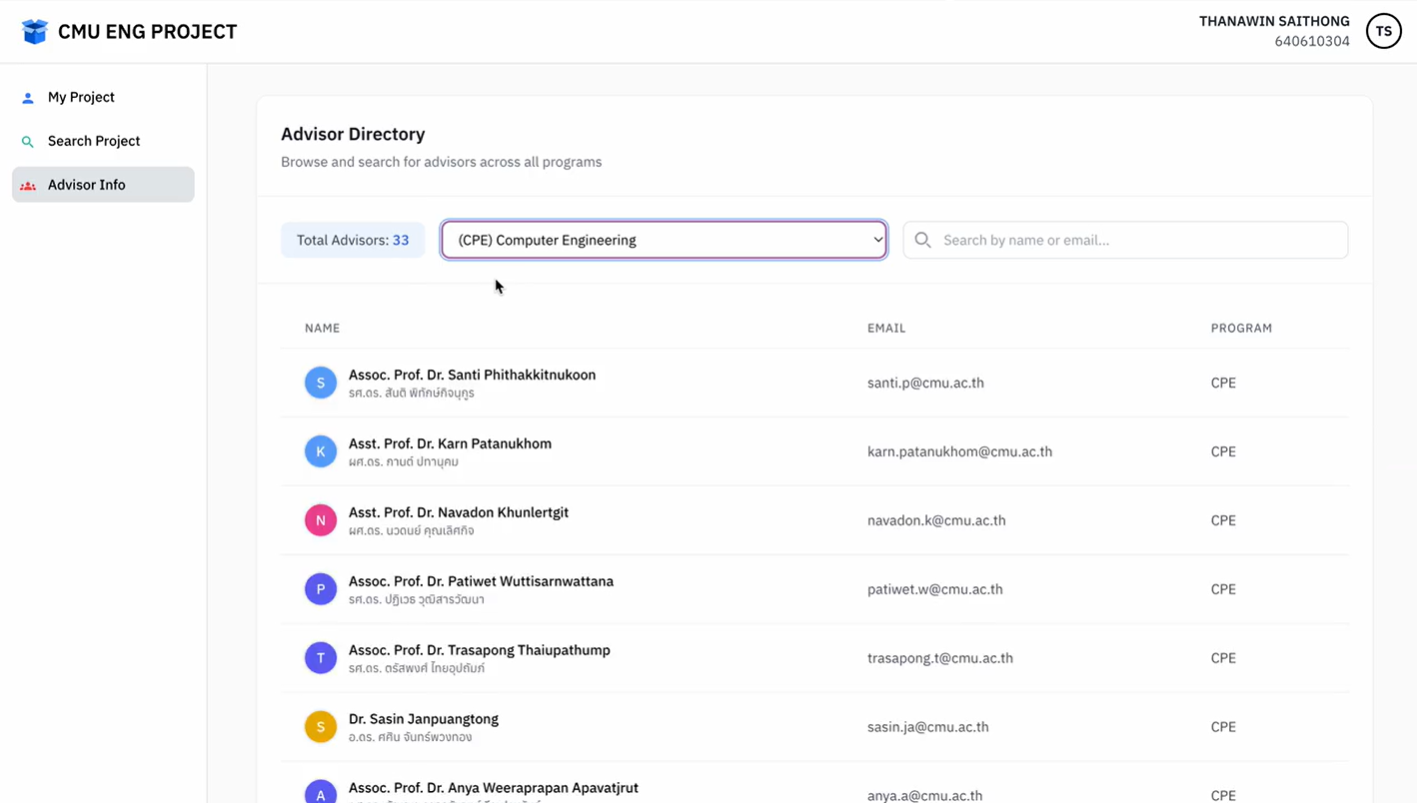
\includegraphics[width=130mm, keepaspectratio ]{pictures/project_box/advisor_info.png}
        \end{figure} 
        \item ดูข้อมูลของอาจารย์ว่าเลยเป็นที่ปรึกษาหรือกรรมการของโครงงานไหนบ้าง
        \begin{figure}[H]
            \centering
            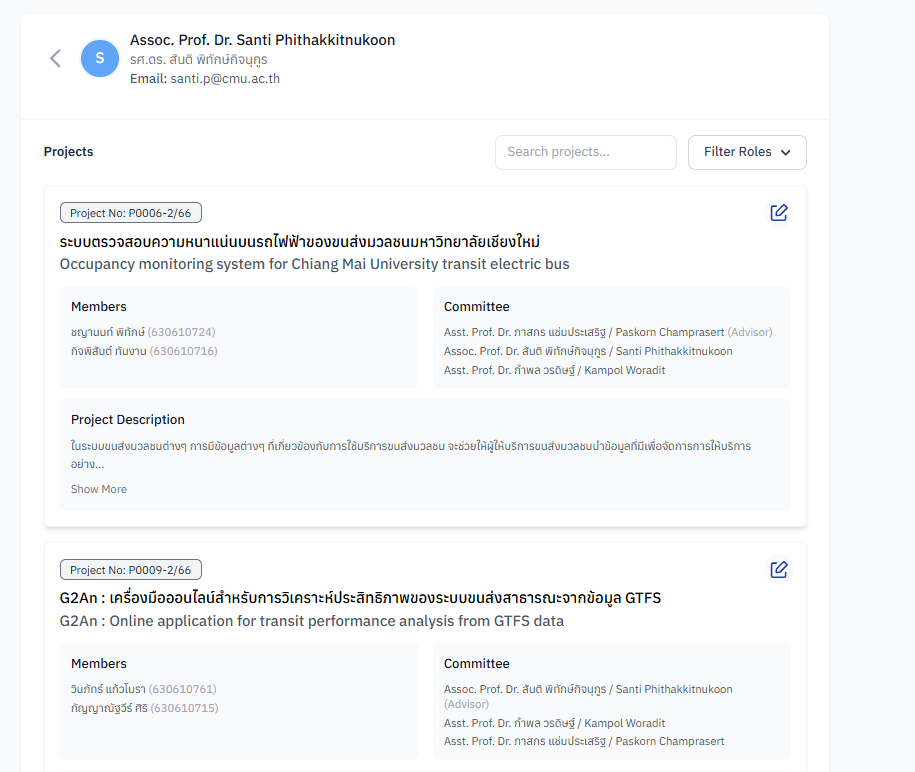
\includegraphics[width=130mm, keepaspectratio ]{pictures/project_box/advisor_project_involvement.png}
        \end{figure} 
    \end{enumerate}
    \item สร้างโครงงาน สามารถสร้างโครงงานใหม่ได้โดยการกดปุ่ม Create Project และกรอกข้อมูลต่างๆที่เกี่ยวข้องกับโครงงาน
    \begin{figure}[H]
        \centering
        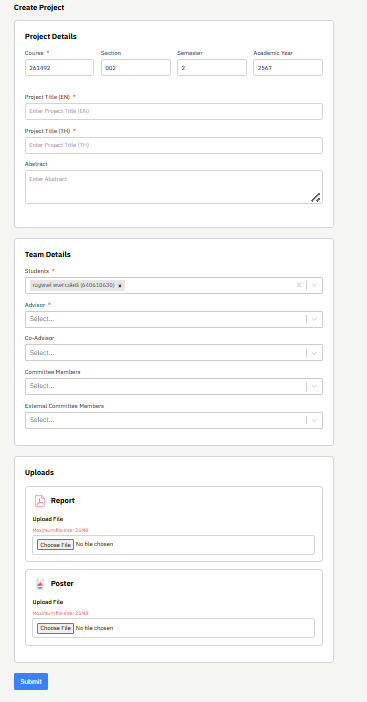
\includegraphics[width=130mm, keepaspectratio ]{pictures/project_box/create_project.png}
    \end{figure} 
\end{enumerate}
\item \textbf{การใช้งานในส่วนของเจ้าหน้าที่ปะจำสาขา Program Admin}
\begin{figure}[H]
    \centering
    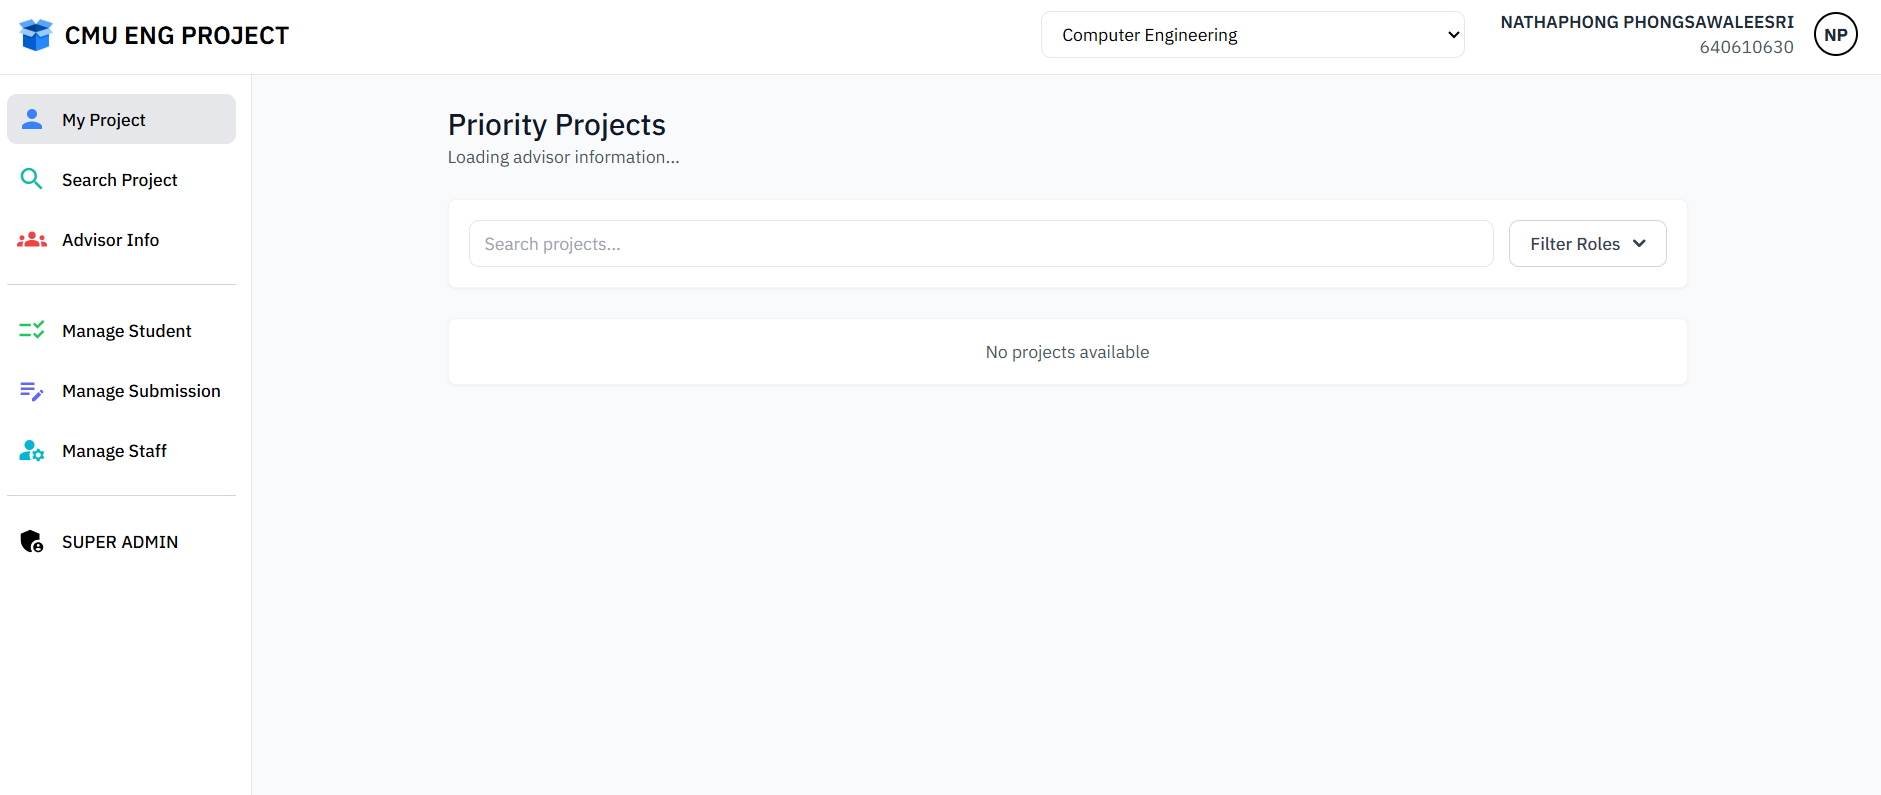
\includegraphics[width=130mm, keepaspectratio ]{pictures/project_box/program_admin_dashboard.png}
\end{figure}
\begin{enumerate}
    \item เลือก Program ที่ต้องการจัดการโครงงาน
    \begin{figure}[H]
        \centering
        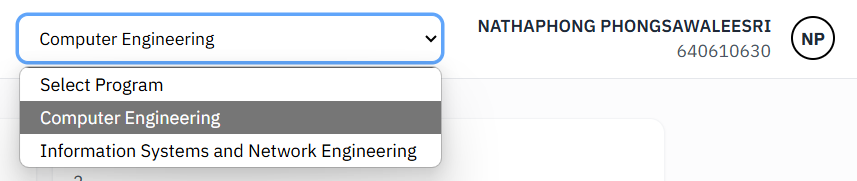
\includegraphics[width=130mm, keepaspectratio ]{pictures/project_box/select_program_before_manage.png}
    \end{figure}
    \item \textbf{จัดการนักศึกษา (Manage Student): } เจ้าหน้าที่สามารถจัดการข้อมูลนักศึกษาและสิทธิ์ในการสร้างโครงงานได้ โดยคลิกที่ปุ่ม "Manage Student" เพื่อเพิ่ม หรือตรวจสอบข้อมูลนักศึกษาว่ามีสิทธิ์ในการสร้างโครงงานในปีการศึกษาและภาคการศึกษานั้นๆ่
    \begin{enumerate}
        \item \textbf{เพิ่มข้อมูลนักศึกษา} เจ้าหน้าที่สามารถเพิ่มรายชื่อนักศึกษาเข้าสู่ระบบได้ โดยการนำเข้าข้อมูลจากไฟล์ Excel ที่ได้จากสำนักทะเบียน
        \begin{figure}[H]
            \centering
            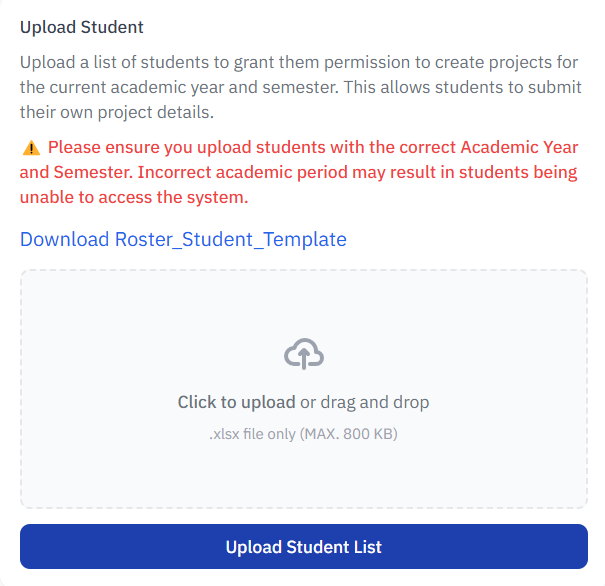
\includegraphics[width=100mm, keepaspectratio ]{pictures/project_box/add_new_student.png}
        \end{figure}
        \begin{figure}[H]
            \centering
            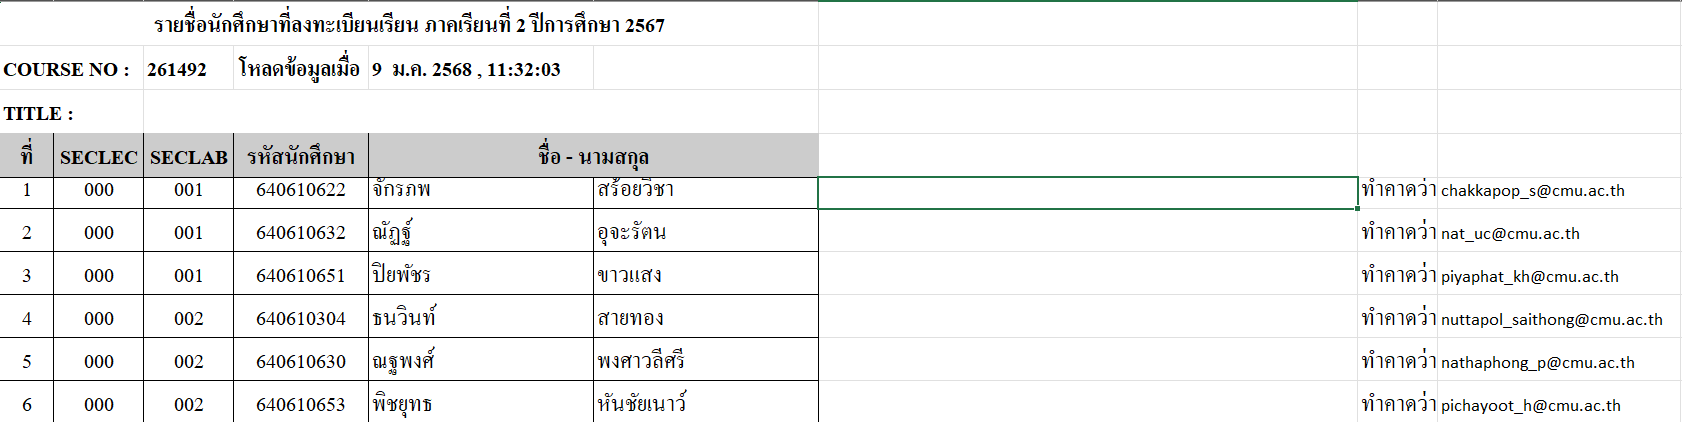
\includegraphics[width=100mm, keepaspectratio ]{pictures/project_box/student_template.png}
            \caption{ตัวอย่างไฟล์ Excel สำหรับนำเข้าข้อมูลนักศึกษา}
        \end{figure}
        \item \textbf{จัดการโครงงาน}: เจ้าหน้าที่สามารถดำเนินการดังนี้
        \begin{enumerate}
            \item \textbf{สร้างโครงงานเก่า}: เพิ่มข้อมูลโครงงานที่นักศึกษาเคยทำไว้แล้วในอดีต
            \item \textbf{มอบหมายโครงงาน}: เพิ่มโครงงานใหม่และกำหนดให้นักศึกษาดำเนินการ โดยนักศึกษาไม่จำเป็นต้องสร้างโครงงานเอง
        \end{enumerate}

        
        \begin{figure}[H]
            \centering
            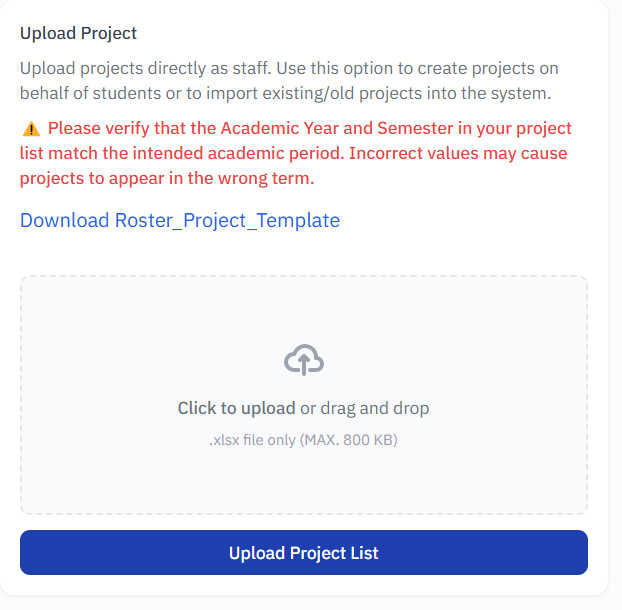
\includegraphics[width=100mm, keepaspectratio ]{pictures/project_box/upload_project_excel.png}
        \end{figure}
        \begin{figure}[H]
            \centering
            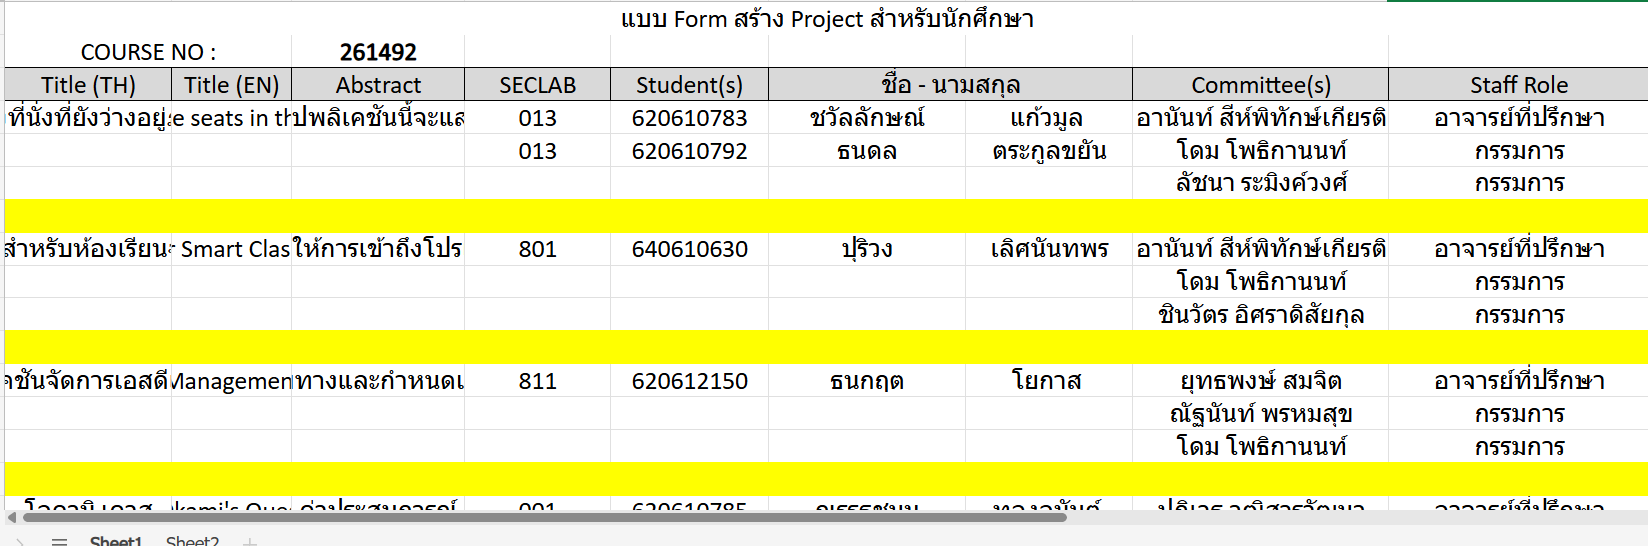
\includegraphics[width=100mm, keepaspectratio ]{pictures/project_box/create_project_template.png}
            \caption{ตัวอย่างไฟล์ Excel สำหรับนำเข้าข้อมูลโครงงาน}
        \end{figure}
    \end{enumerate}

    \newpage
    \item \textbf{จัดการรูปแบบการส่งโครงงาน (Manage Submission): } เจ้าหน้าที่สามารถกำหนดรูปแบบการส่งโครงงานให้กับนักศึกษาได้
    \begin{figure}[H]
        \centering
        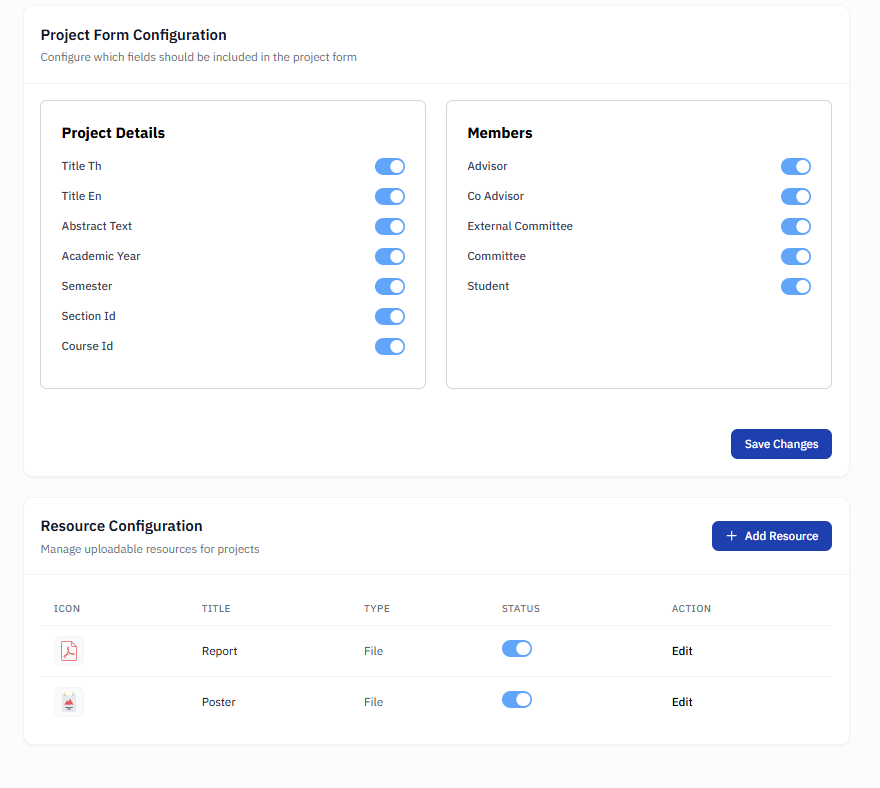
\includegraphics[width=100mm, keepaspectratio ]{pictures/project_box/project_submission_1.png}
        \caption{รูปแบบการส่งโครงงาน}
    \end{figure}

    \begin{figure}[H]
        \centering
        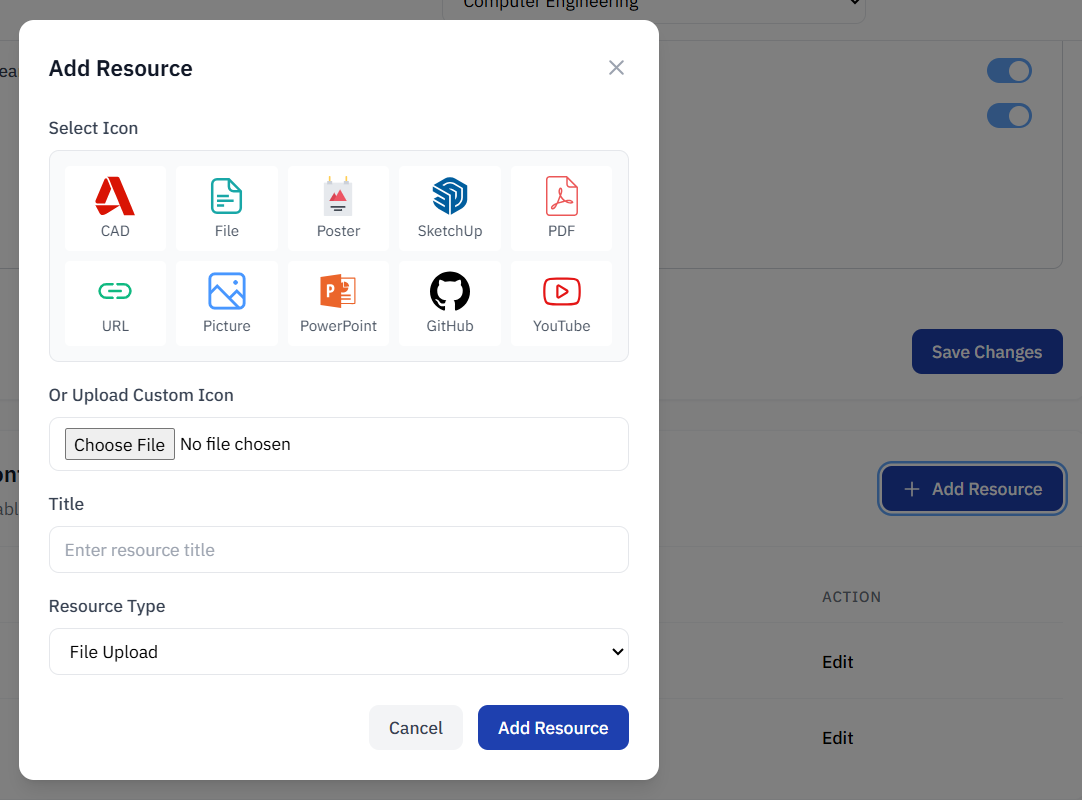
\includegraphics[width=100mm, keepaspectratio ]{pictures/project_box/project_submission_2.png}
        \caption{กำหนดสิ่งที่นักศึกษาต้องส่งในโครงงานของแต่ละสาขา เช่น รายงาน, โค้ด, ฯลฯ}
    \end{figure}
    \newpage
    \item \textbf{จัดการตณาอาจารย์ในสาขา (Manage Staff): } เจ้าหน้าที่สามารถจัดการข้อมูลของอาจารย์ในสาขาได้
    \begin{figure}[H]
        \centering
        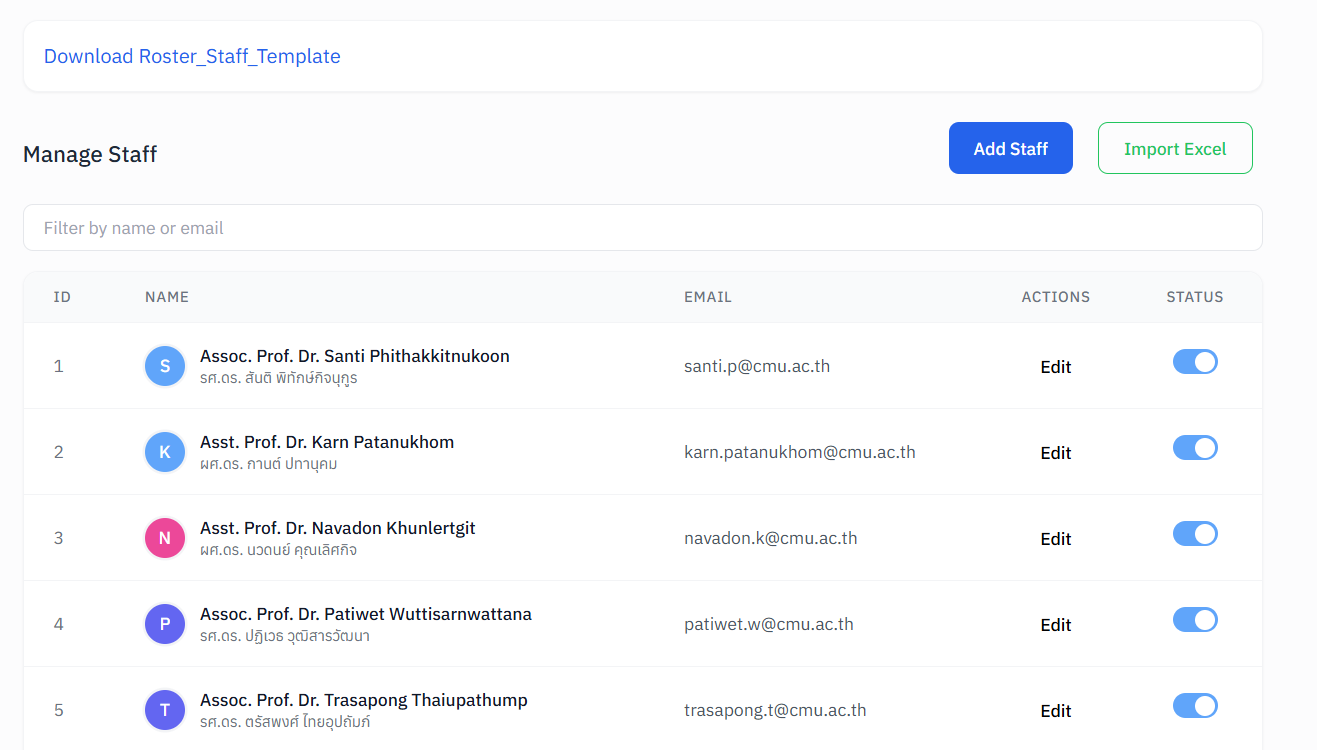
\includegraphics[width=100mm, keepaspectratio ]{pictures/project_box/staff_list.png}
    \end{figure}
    \begin{figure}[H]
        \centering
        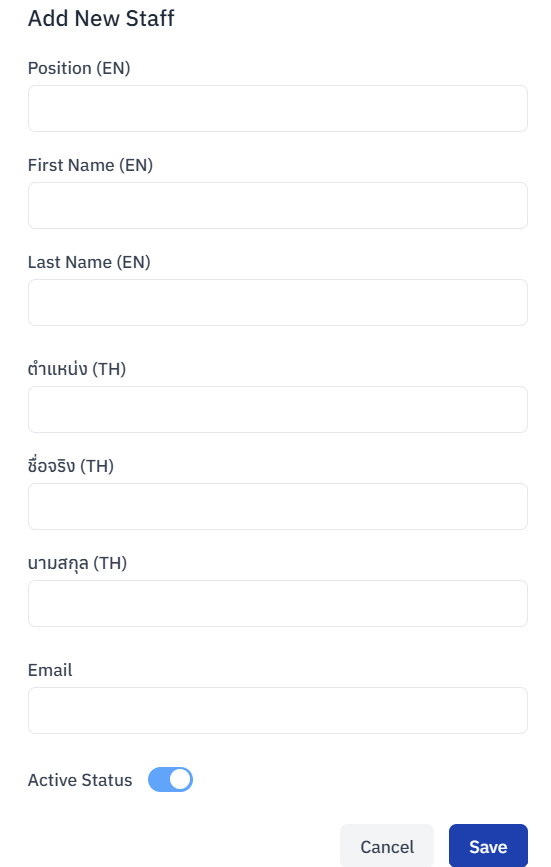
\includegraphics[width=100mm, keepaspectratio ]{pictures/project_box/add_staff.png}
    \end{figure}
    \begin{figure}[H]
        \centering
        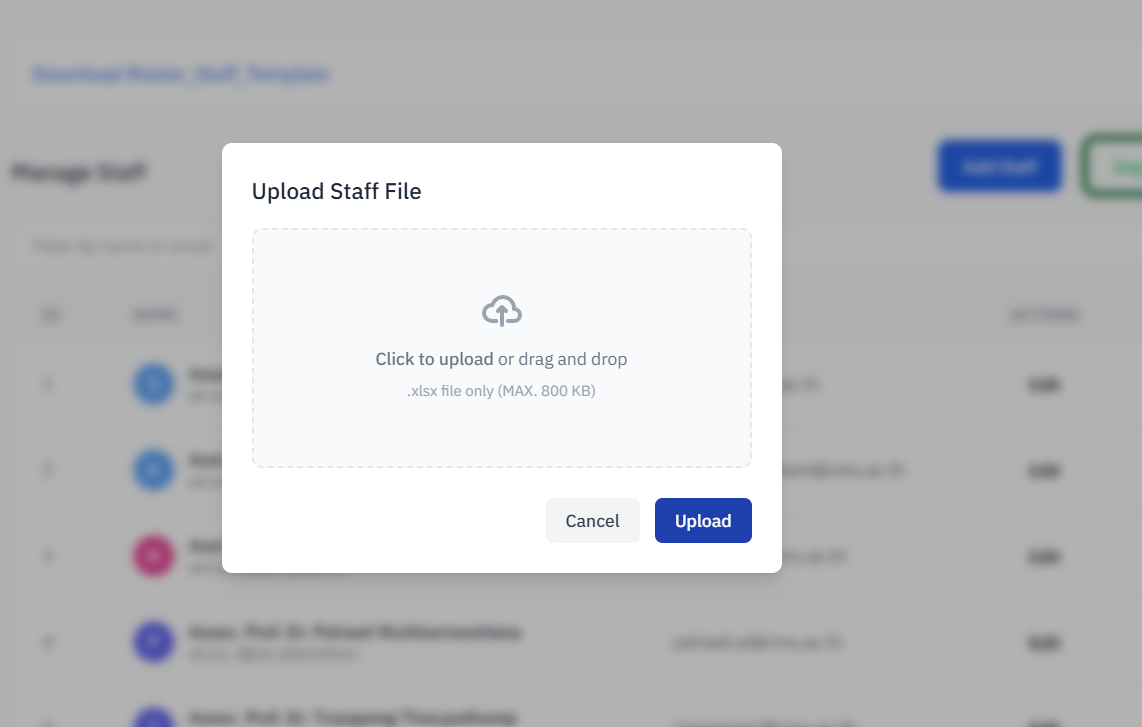
\includegraphics[width=100mm, keepaspectratio ]{pictures/project_box/add_staff_excel.png}
        \caption{ตัวอย่างไฟล์ Excel สำหรับนำเข้าข้อมูลอาจารย์}
    \end{figure}
    \begin{figure}
        \centering
        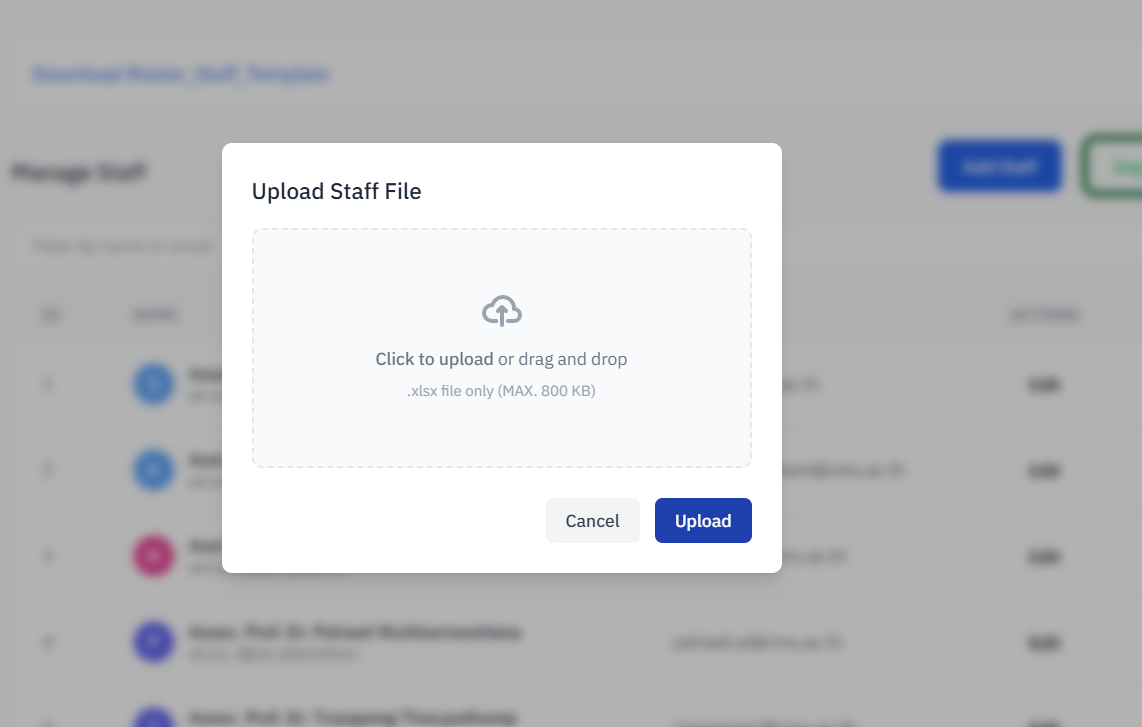
\includegraphics[width=100mm, keepaspectratio ]{pictures/project_box/add_staff_excel.png}
        \caption{เพิ่มข้อมูลอาจารย์ โดยการนำเข้าข้อมูลจากไฟล์ Excel ที่ได้จากสำนักทะเบียน} 
    \end{figure}
    \begin{figure}[H]
        \centering
        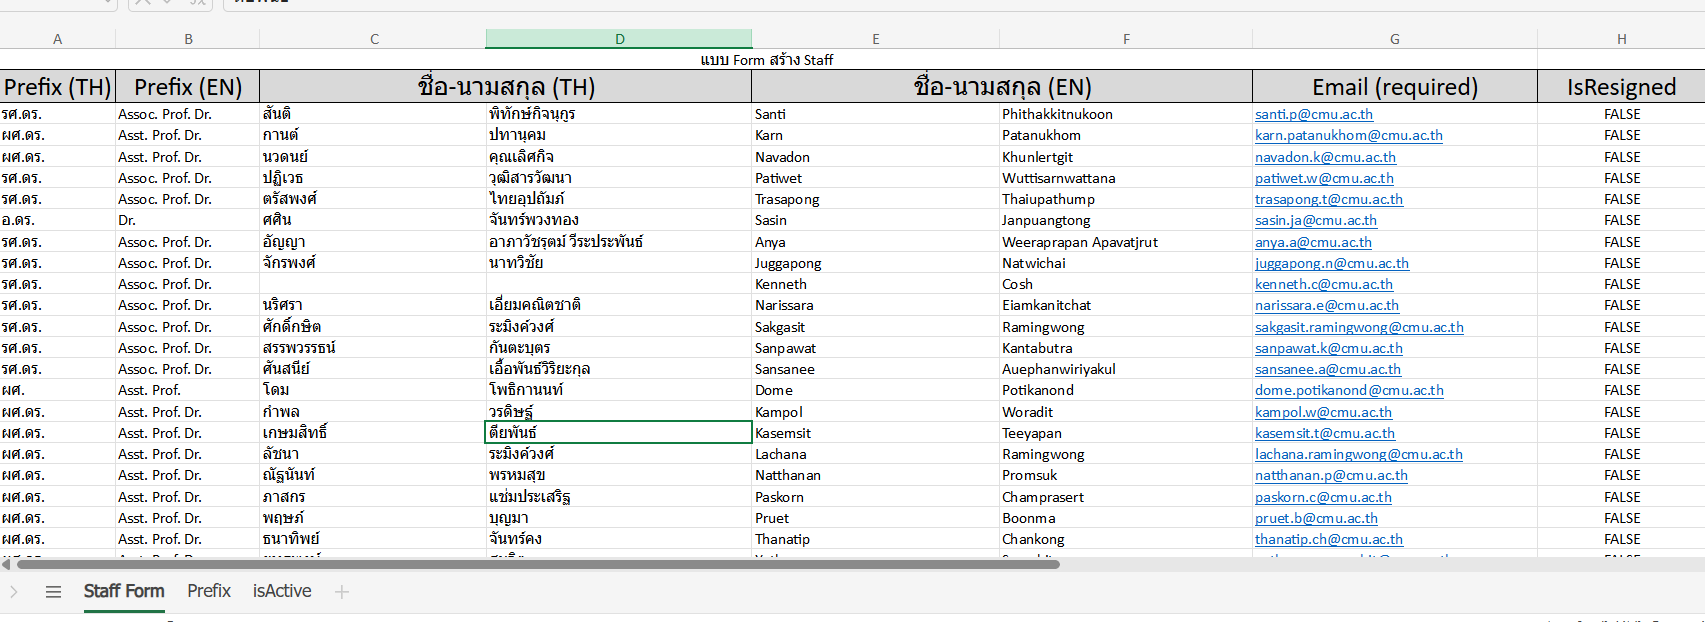
\includegraphics[width=140mm, keepaspectratio ]{pictures/project_box/staff_excel_template.png}
        \caption{ตัวอย่างไฟล์ Excel สำหรับนำเข้าข้อมูลอาจารย์} 
    \end{figure}   
\end{enumerate}
\newpage
\item \textbf{ผู้ดูแลระบบแพลตฟอร์ม (Super Admin): } สามารถจัดการข้อมูลของสาขาและโครงงานทั้งหมดในระบบ รวมถึงจัดการสิทธิ์ให้กับเจ้าหน้าที่ประจำสาขา
\begin{figure}
    \centering
    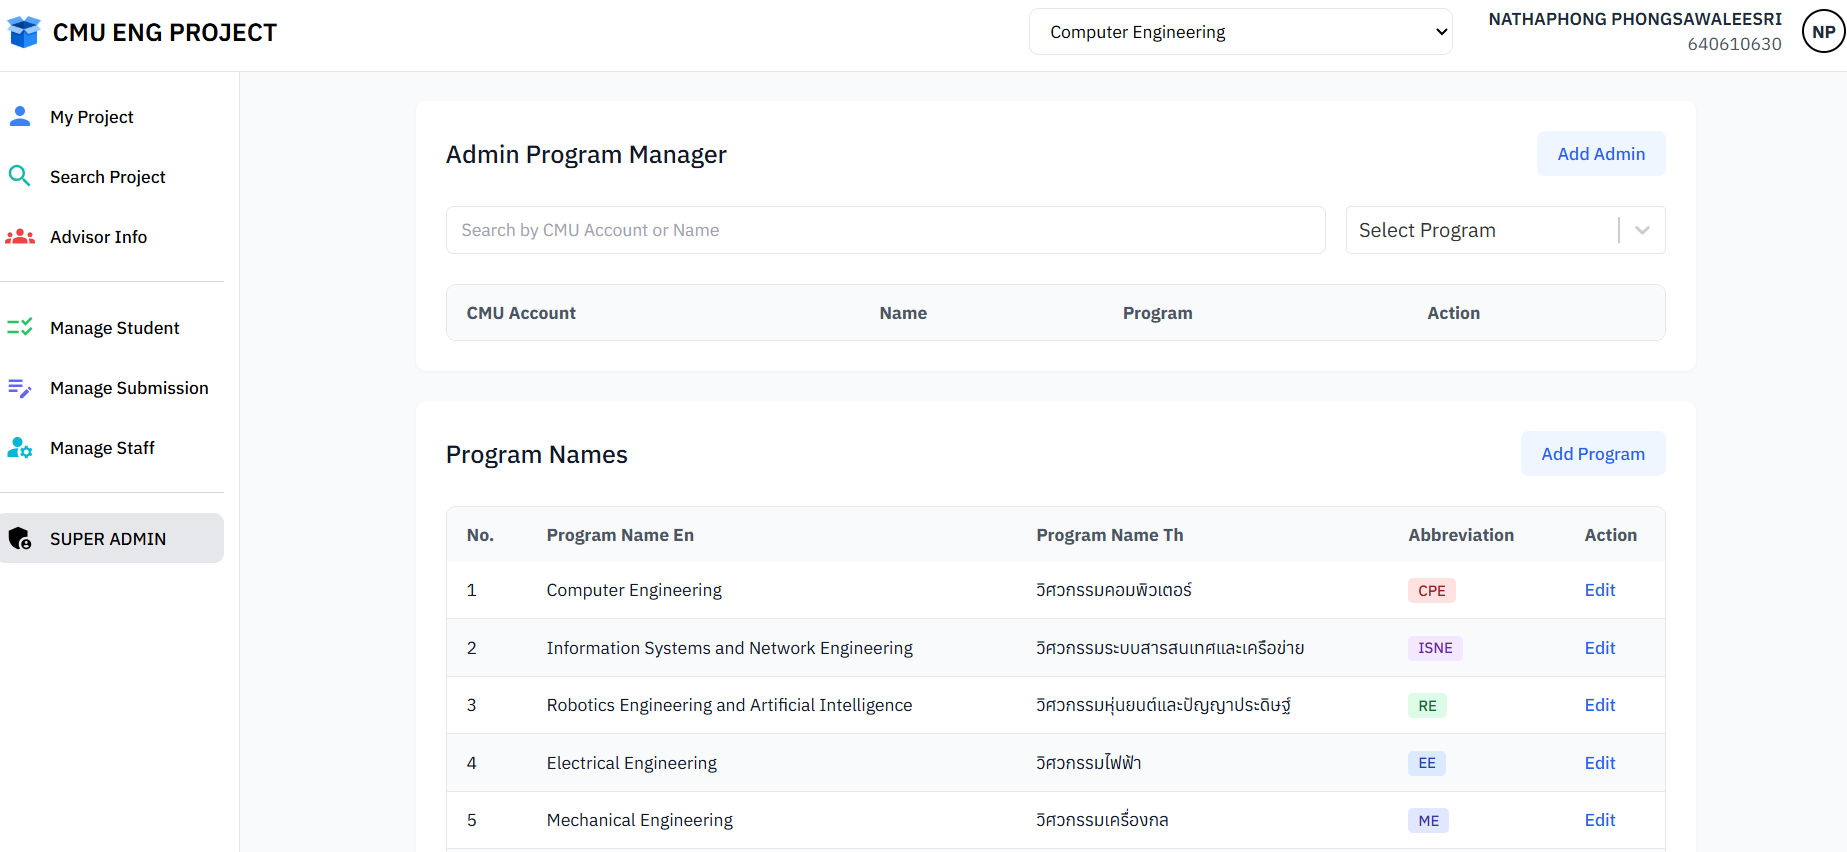
\includegraphics[width=130mm, keepaspectratio ]{pictures/project_box/super_admin.png}
\end{figure}
\begin{figure}[H]
    \centering
    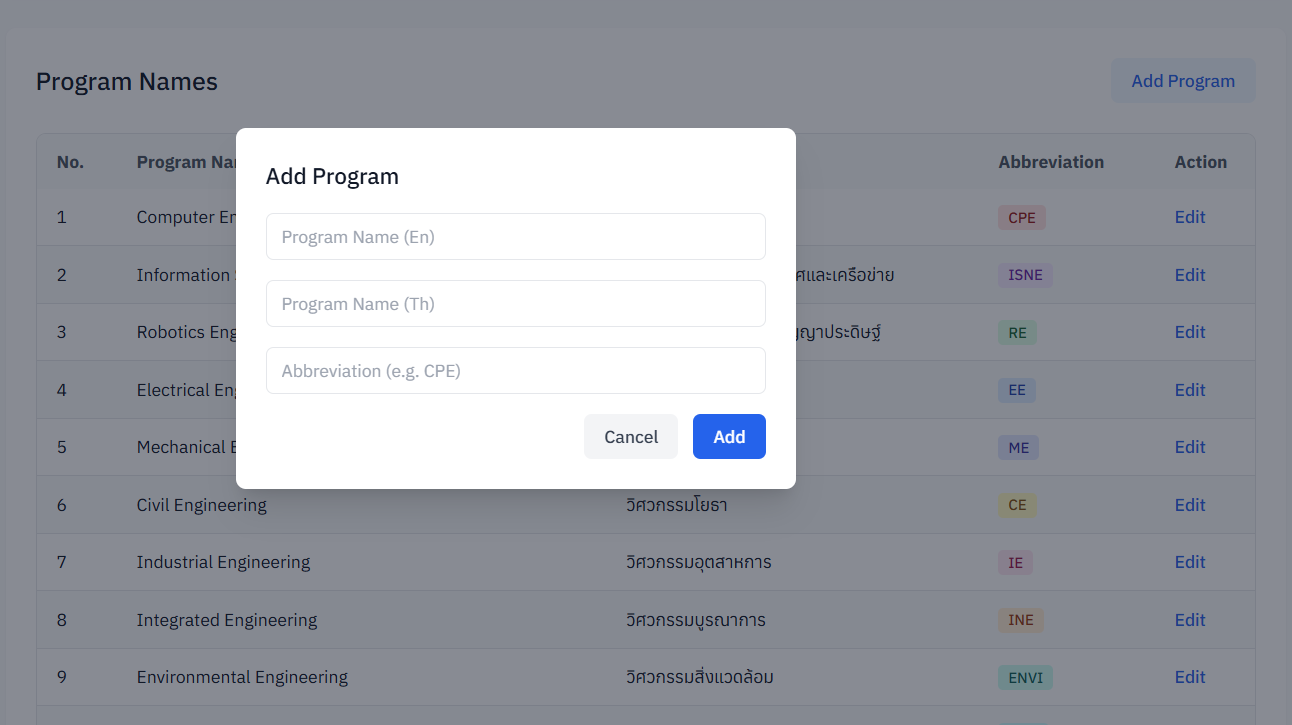
\includegraphics[width=130mm, keepaspectratio ]{pictures/project_box/manage_program.png}
    \caption{จัดการข้อมูลสาขา}
\end{figure}
\begin{figure}[H]
    \centering
    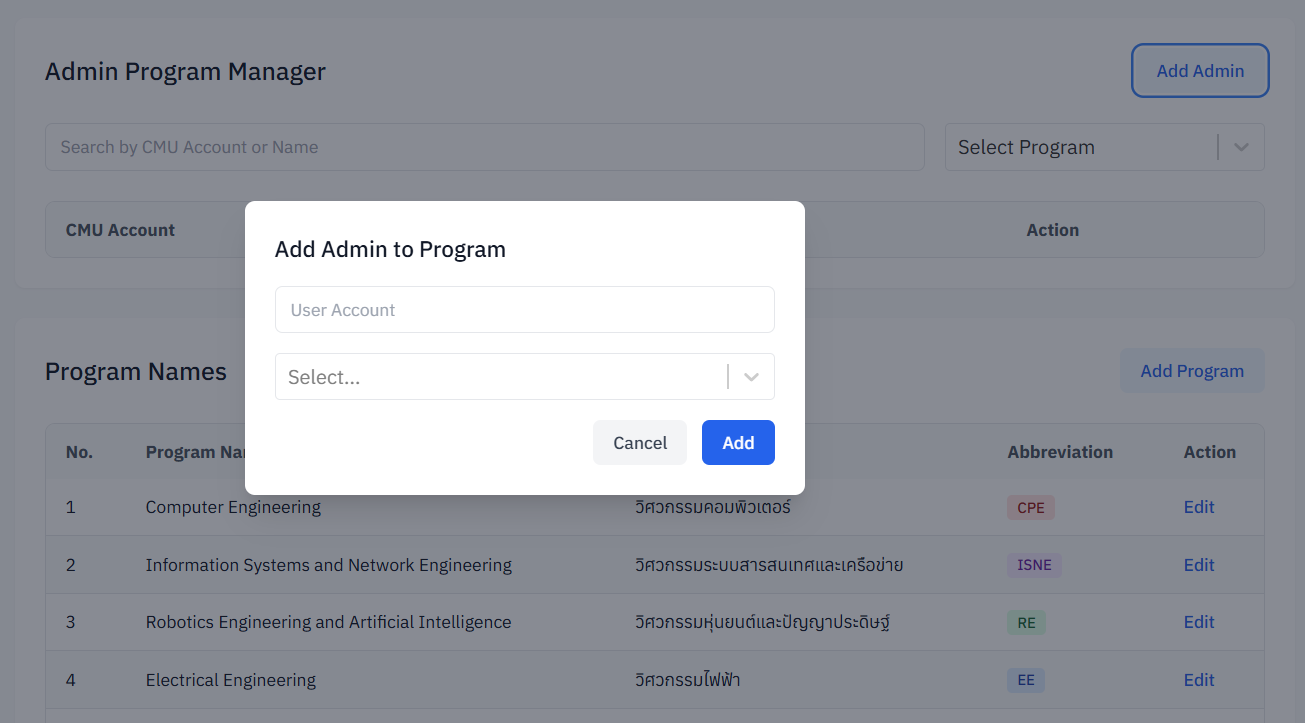
\includegraphics[width=130mm, keepaspectratio ]{pictures/project_box/add_program_admin.png}
    \caption{เพิ่มเจ้าหน้าที่ประจำสาขา}
\end{figure}
\end{itemize}
% \section{appendix}
